\documentclass[]{article}
\usepackage{lmodern}
\usepackage{amssymb,amsmath}
\usepackage{ifxetex,ifluatex}
\usepackage{fixltx2e} % provides \textsubscript
\ifnum 0\ifxetex 1\fi\ifluatex 1\fi=0 % if pdftex
  \usepackage[T1]{fontenc}
  \usepackage[utf8]{inputenc}
\else % if luatex or xelatex
  \ifxetex
    \usepackage{mathspec}
  \else
    \usepackage{fontspec}
  \fi
  \defaultfontfeatures{Ligatures=TeX,Scale=MatchLowercase}
\fi
% use upquote if available, for straight quotes in verbatim environments
\IfFileExists{upquote.sty}{\usepackage{upquote}}{}
% use microtype if available
\IfFileExists{microtype.sty}{%
\usepackage{microtype}
\UseMicrotypeSet[protrusion]{basicmath} % disable protrusion for tt fonts
}{}
\usepackage[margin=1in]{geometry}
\usepackage{hyperref}
\hypersetup{unicode=true,
            pdftitle={Class 8 machine learning},
            pdfauthor={Hongji Jiang},
            pdfborder={0 0 0},
            breaklinks=true}
\urlstyle{same}  % don't use monospace font for urls
\usepackage{color}
\usepackage{fancyvrb}
\newcommand{\VerbBar}{|}
\newcommand{\VERB}{\Verb[commandchars=\\\{\}]}
\DefineVerbatimEnvironment{Highlighting}{Verbatim}{commandchars=\\\{\}}
% Add ',fontsize=\small' for more characters per line
\usepackage{framed}
\definecolor{shadecolor}{RGB}{248,248,248}
\newenvironment{Shaded}{\begin{snugshade}}{\end{snugshade}}
\newcommand{\KeywordTok}[1]{\textcolor[rgb]{0.13,0.29,0.53}{\textbf{#1}}}
\newcommand{\DataTypeTok}[1]{\textcolor[rgb]{0.13,0.29,0.53}{#1}}
\newcommand{\DecValTok}[1]{\textcolor[rgb]{0.00,0.00,0.81}{#1}}
\newcommand{\BaseNTok}[1]{\textcolor[rgb]{0.00,0.00,0.81}{#1}}
\newcommand{\FloatTok}[1]{\textcolor[rgb]{0.00,0.00,0.81}{#1}}
\newcommand{\ConstantTok}[1]{\textcolor[rgb]{0.00,0.00,0.00}{#1}}
\newcommand{\CharTok}[1]{\textcolor[rgb]{0.31,0.60,0.02}{#1}}
\newcommand{\SpecialCharTok}[1]{\textcolor[rgb]{0.00,0.00,0.00}{#1}}
\newcommand{\StringTok}[1]{\textcolor[rgb]{0.31,0.60,0.02}{#1}}
\newcommand{\VerbatimStringTok}[1]{\textcolor[rgb]{0.31,0.60,0.02}{#1}}
\newcommand{\SpecialStringTok}[1]{\textcolor[rgb]{0.31,0.60,0.02}{#1}}
\newcommand{\ImportTok}[1]{#1}
\newcommand{\CommentTok}[1]{\textcolor[rgb]{0.56,0.35,0.01}{\textit{#1}}}
\newcommand{\DocumentationTok}[1]{\textcolor[rgb]{0.56,0.35,0.01}{\textbf{\textit{#1}}}}
\newcommand{\AnnotationTok}[1]{\textcolor[rgb]{0.56,0.35,0.01}{\textbf{\textit{#1}}}}
\newcommand{\CommentVarTok}[1]{\textcolor[rgb]{0.56,0.35,0.01}{\textbf{\textit{#1}}}}
\newcommand{\OtherTok}[1]{\textcolor[rgb]{0.56,0.35,0.01}{#1}}
\newcommand{\FunctionTok}[1]{\textcolor[rgb]{0.00,0.00,0.00}{#1}}
\newcommand{\VariableTok}[1]{\textcolor[rgb]{0.00,0.00,0.00}{#1}}
\newcommand{\ControlFlowTok}[1]{\textcolor[rgb]{0.13,0.29,0.53}{\textbf{#1}}}
\newcommand{\OperatorTok}[1]{\textcolor[rgb]{0.81,0.36,0.00}{\textbf{#1}}}
\newcommand{\BuiltInTok}[1]{#1}
\newcommand{\ExtensionTok}[1]{#1}
\newcommand{\PreprocessorTok}[1]{\textcolor[rgb]{0.56,0.35,0.01}{\textit{#1}}}
\newcommand{\AttributeTok}[1]{\textcolor[rgb]{0.77,0.63,0.00}{#1}}
\newcommand{\RegionMarkerTok}[1]{#1}
\newcommand{\InformationTok}[1]{\textcolor[rgb]{0.56,0.35,0.01}{\textbf{\textit{#1}}}}
\newcommand{\WarningTok}[1]{\textcolor[rgb]{0.56,0.35,0.01}{\textbf{\textit{#1}}}}
\newcommand{\AlertTok}[1]{\textcolor[rgb]{0.94,0.16,0.16}{#1}}
\newcommand{\ErrorTok}[1]{\textcolor[rgb]{0.64,0.00,0.00}{\textbf{#1}}}
\newcommand{\NormalTok}[1]{#1}
\usepackage{graphicx,grffile}
\makeatletter
\def\maxwidth{\ifdim\Gin@nat@width>\linewidth\linewidth\else\Gin@nat@width\fi}
\def\maxheight{\ifdim\Gin@nat@height>\textheight\textheight\else\Gin@nat@height\fi}
\makeatother
% Scale images if necessary, so that they will not overflow the page
% margins by default, and it is still possible to overwrite the defaults
% using explicit options in \includegraphics[width, height, ...]{}
\setkeys{Gin}{width=\maxwidth,height=\maxheight,keepaspectratio}
\IfFileExists{parskip.sty}{%
\usepackage{parskip}
}{% else
\setlength{\parindent}{0pt}
\setlength{\parskip}{6pt plus 2pt minus 1pt}
}
\setlength{\emergencystretch}{3em}  % prevent overfull lines
\providecommand{\tightlist}{%
  \setlength{\itemsep}{0pt}\setlength{\parskip}{0pt}}
\setcounter{secnumdepth}{0}
% Redefines (sub)paragraphs to behave more like sections
\ifx\paragraph\undefined\else
\let\oldparagraph\paragraph
\renewcommand{\paragraph}[1]{\oldparagraph{#1}\mbox{}}
\fi
\ifx\subparagraph\undefined\else
\let\oldsubparagraph\subparagraph
\renewcommand{\subparagraph}[1]{\oldsubparagraph{#1}\mbox{}}
\fi

%%% Use protect on footnotes to avoid problems with footnotes in titles
\let\rmarkdownfootnote\footnote%
\def\footnote{\protect\rmarkdownfootnote}

%%% Change title format to be more compact
\usepackage{titling}

% Create subtitle command for use in maketitle
\providecommand{\subtitle}[1]{
  \posttitle{
    \begin{center}\large#1\end{center}
    }
}

\setlength{\droptitle}{-2em}

  \title{Class 8 machine learning}
    \pretitle{\vspace{\droptitle}\centering\huge}
  \posttitle{\par}
    \author{Hongji Jiang}
    \preauthor{\centering\large\emph}
  \postauthor{\par}
      \predate{\centering\large\emph}
  \postdate{\par}
    \date{10/24/2019}


\begin{document}
\maketitle

\subsection{K-means Clustering}\label{k-means-clustering}

\begin{Shaded}
\begin{Highlighting}[]
 \CommentTok{# Generate some example data for clustering}
\NormalTok{tmp <-}\StringTok{ }\KeywordTok{c}\NormalTok{(}\KeywordTok{rnorm}\NormalTok{(}\DecValTok{30}\NormalTok{,}\OperatorTok{-}\DecValTok{3}\NormalTok{), }\KeywordTok{rnorm}\NormalTok{(}\DecValTok{30}\NormalTok{,}\DecValTok{3}\NormalTok{))}
\NormalTok{x <-}\StringTok{ }\KeywordTok{cbind}\NormalTok{(}\DataTypeTok{x=}\NormalTok{tmp, }\DataTypeTok{y=}\KeywordTok{rev}\NormalTok{(tmp))}
\KeywordTok{plot}\NormalTok{(x)}
\end{Highlighting}
\end{Shaded}

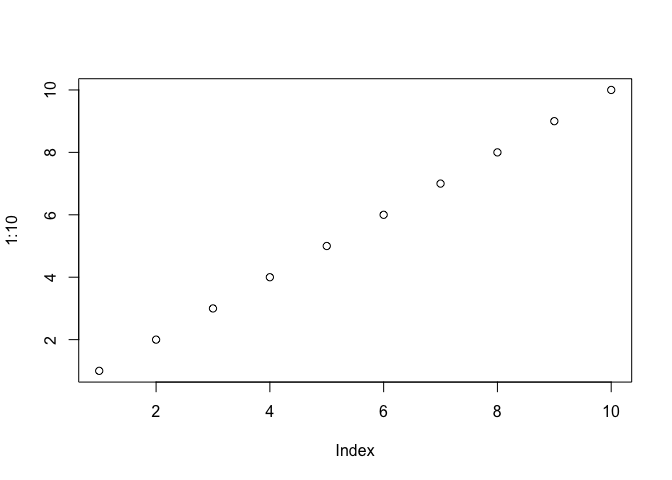
\includegraphics{class8_files/figure-latex/unnamed-chunk-1-1.pdf}

Q. How many points are in each cluster? Q. What `component' of your
result object details - cluster size? - cluster assignment/membership? -
cluster center?

\begin{Shaded}
\begin{Highlighting}[]
\NormalTok{k <-}\StringTok{ }\KeywordTok{kmeans}\NormalTok{(x, }\DataTypeTok{centers=}\DecValTok{2}\NormalTok{, }\DataTypeTok{nstart=}\DecValTok{20}\NormalTok{)}
\NormalTok{k}\OperatorTok{$}\NormalTok{size}
\end{Highlighting}
\end{Shaded}

\begin{verbatim}
## [1] 30 30
\end{verbatim}

\begin{Shaded}
\begin{Highlighting}[]
\NormalTok{k}\OperatorTok{$}\NormalTok{cluster}
\end{Highlighting}
\end{Shaded}

\begin{verbatim}
##  [1] 2 2 2 2 2 2 2 2 2 2 2 2 2 2 2 2 2 2 2 2 2 2 2 2 2 2 2 2 2 2 1 1 1 1 1
## [36] 1 1 1 1 1 1 1 1 1 1 1 1 1 1 1 1 1 1 1 1 1 1 1 1 1
\end{verbatim}

\begin{Shaded}
\begin{Highlighting}[]
\NormalTok{k}\OperatorTok{$}\NormalTok{centers}
\end{Highlighting}
\end{Shaded}

\begin{verbatim}
##           x         y
## 1  2.801471 -3.358177
## 2 -3.358177  2.801471
\end{verbatim}

Plot x colored by the kmeans cluster assignment and add cluster centers
as blue points

\begin{Shaded}
\begin{Highlighting}[]
\KeywordTok{plot}\NormalTok{(x, }\DataTypeTok{col =}\NormalTok{ k}\OperatorTok{$}\NormalTok{cluster)}
\KeywordTok{points}\NormalTok{(k}\OperatorTok{$}\NormalTok{centers,}\DataTypeTok{col =} \DecValTok{12}\NormalTok{,}\DataTypeTok{pch =} \DecValTok{15}\NormalTok{)}
\end{Highlighting}
\end{Shaded}

\includegraphics{class8_files/figure-latex/unnamed-chunk-3-1.pdf}

\subsection{Hierarchical clustering in
R}\label{hierarchical-clustering-in-r}

The `hclust()' function requires a distance matrix as input You can get
this from `dist()' function

\begin{Shaded}
\begin{Highlighting}[]
\CommentTok{# First we need to calculate point (dis)similarity}
\CommentTok{#   as the Euclidean distance between observations}
\NormalTok{dist_matrix <-}\StringTok{ }\KeywordTok{dist}\NormalTok{(x)}
\CommentTok{# The hclust() function returns a hierarchical}
\CommentTok{#  clustering model}
\NormalTok{hc <-}\StringTok{ }\KeywordTok{hclust}\NormalTok{(}\DataTypeTok{d =}\NormalTok{ dist_matrix)}
\CommentTok{# the print method is not so useful here}
\NormalTok{hc}
\end{Highlighting}
\end{Shaded}

\begin{verbatim}
## 
## Call:
## hclust(d = dist_matrix)
## 
## Cluster method   : complete 
## Distance         : euclidean 
## Number of objects: 60
\end{verbatim}

\begin{Shaded}
\begin{Highlighting}[]
\KeywordTok{plot}\NormalTok{(hc)}
\KeywordTok{abline}\NormalTok{(}\DataTypeTok{h=}\DecValTok{6}\NormalTok{,}\DataTypeTok{col=}\StringTok{'red'}\NormalTok{)}
\end{Highlighting}
\end{Shaded}

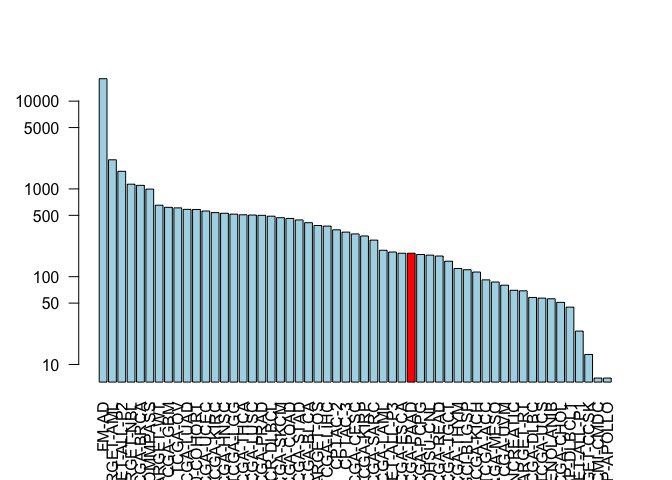
\includegraphics{class8_files/figure-latex/unnamed-chunk-5-1.pdf}

\begin{Shaded}
\begin{Highlighting}[]
\KeywordTok{cutree}\NormalTok{(hc,}\DataTypeTok{h=}\DecValTok{6}\NormalTok{)}
\end{Highlighting}
\end{Shaded}

\begin{verbatim}
##  [1] 1 1 1 1 1 1 1 1 1 1 1 1 1 1 1 1 1 1 1 1 1 1 1 1 1 1 1 1 1 1 2 2 2 2 2
## [36] 2 2 2 2 2 2 2 2 2 2 2 2 2 2 2 2 2 2 2 2 2 2 2 2 2
\end{verbatim}

\begin{Shaded}
\begin{Highlighting}[]
 \CommentTok{# Step 1. Generate some example data for clustering}
\NormalTok{x <-}\StringTok{ }\KeywordTok{rbind}\NormalTok{(}
  \KeywordTok{matrix}\NormalTok{(}\KeywordTok{rnorm}\NormalTok{(}\DecValTok{100}\NormalTok{, }\DataTypeTok{mean=}\DecValTok{0}\NormalTok{, }\DataTypeTok{sd =} \FloatTok{0.3}\NormalTok{), }\DataTypeTok{ncol =} \DecValTok{2}\NormalTok{),   }\CommentTok{# c1}
  \KeywordTok{matrix}\NormalTok{(}\KeywordTok{rnorm}\NormalTok{(}\DecValTok{100}\NormalTok{, }\DataTypeTok{mean =} \DecValTok{1}\NormalTok{, }\DataTypeTok{sd =} \FloatTok{0.3}\NormalTok{), }\DataTypeTok{ncol =} \DecValTok{2}\NormalTok{), }\CommentTok{# c2}
  \KeywordTok{matrix}\NormalTok{(}\KeywordTok{c}\NormalTok{(}\KeywordTok{rnorm}\NormalTok{(}\DecValTok{50}\NormalTok{, }\DataTypeTok{mean =} \DecValTok{1}\NormalTok{, }\DataTypeTok{sd =} \FloatTok{0.3}\NormalTok{),           }\CommentTok{# c3}
           \KeywordTok{rnorm}\NormalTok{(}\DecValTok{50}\NormalTok{, }\DataTypeTok{mean =} \DecValTok{0}\NormalTok{, }\DataTypeTok{sd =} \FloatTok{0.3}\NormalTok{)), }\DataTypeTok{ncol =} \DecValTok{2}\NormalTok{))}
\KeywordTok{colnames}\NormalTok{(x) <-}\StringTok{ }\KeywordTok{c}\NormalTok{(}\StringTok{"x"}\NormalTok{, }\StringTok{"y"}\NormalTok{)}
\CommentTok{# Step 2. Plot the data without clustering}
\KeywordTok{plot}\NormalTok{(x)}
\end{Highlighting}
\end{Shaded}

\includegraphics{class8_files/figure-latex/unnamed-chunk-6-1.pdf}

\begin{Shaded}
\begin{Highlighting}[]
\CommentTok{# Step 3. Generate colors for known clusters}
\CommentTok{#         (just so we can compare to hclust results)}
\NormalTok{col <-}\StringTok{ }\KeywordTok{as.factor}\NormalTok{( }\KeywordTok{rep}\NormalTok{(}\KeywordTok{c}\NormalTok{(}\StringTok{"c1"}\NormalTok{,}\StringTok{"c2"}\NormalTok{,}\StringTok{"c3"}\NormalTok{), }\DataTypeTok{each=}\DecValTok{50}\NormalTok{) )}
\KeywordTok{plot}\NormalTok{(x, }\DataTypeTok{col=}\NormalTok{col)}
\end{Highlighting}
\end{Shaded}

\includegraphics{class8_files/figure-latex/unnamed-chunk-6-2.pdf}

\begin{Shaded}
\begin{Highlighting}[]
\KeywordTok{kmeans}\NormalTok{(x,}\DataTypeTok{centers=}\DecValTok{3}\NormalTok{,}\DataTypeTok{nstart =}\DecValTok{20}\NormalTok{)}
\end{Highlighting}
\end{Shaded}

\begin{verbatim}
## K-means clustering with 3 clusters of sizes 46, 56, 48
## 
## Cluster means:
##             x            y
## 1 -0.08121386 -0.008521267
## 2  0.97593480  0.993375591
## 3  0.97041920 -0.191999748
## 
## Clustering vector:
##   [1] 1 1 1 1 1 1 1 1 1 1 1 1 1 1 1 1 1 2 1 3 1 1 1 1 2 1 1 1 1 1 3 1 1 1 1
##  [36] 1 1 1 1 1 1 1 1 1 3 1 1 1 1 1 2 2 2 2 2 2 2 2 2 2 2 2 2 2 2 2 2 2 2 2
##  [71] 2 2 2 2 2 2 2 2 2 2 2 2 2 2 2 2 2 2 2 2 2 2 2 2 2 2 2 2 2 2 3 3 3 3 3
## [106] 3 3 3 3 3 3 3 3 3 3 3 2 3 3 3 3 3 3 3 1 3 2 3 3 3 3 3 3 3 3 3 3 3 3 3
## [141] 3 2 3 3 2 3 3 3 3 3
## 
## Within cluster sum of squares by cluster:
## [1]  7.037250 11.625654  8.593182
##  (between_SS / total_SS =  74.2 %)
## 
## Available components:
## 
## [1] "cluster"      "centers"      "totss"        "withinss"    
## [5] "tot.withinss" "betweenss"    "size"         "iter"        
## [9] "ifault"
\end{verbatim}

\begin{Shaded}
\begin{Highlighting}[]
\CommentTok{#clustering}
\NormalTok{hc <-}\StringTok{ }\KeywordTok{hclust}\NormalTok{(}\KeywordTok{dist}\NormalTok{(x))}

\CommentTok{#draw tree}
\KeywordTok{plot}\NormalTok{(hc)}
\KeywordTok{abline}\NormalTok{(}\DataTypeTok{h=}\DecValTok{2}\NormalTok{,}\DataTypeTok{col=}\StringTok{'red'}\NormalTok{)}
\end{Highlighting}
\end{Shaded}

\includegraphics{class8_files/figure-latex/unnamed-chunk-8-1.pdf}

\begin{Shaded}
\begin{Highlighting}[]
\CommentTok{#cut the tree into clusters/grps}
\NormalTok{grps <-}\StringTok{ }\KeywordTok{cutree}\NormalTok{(hc,}\DataTypeTok{h=}\DecValTok{2}\NormalTok{)}
\NormalTok{grps}
\end{Highlighting}
\end{Shaded}

\begin{verbatim}
##   [1] 1 1 1 1 1 1 1 1 1 1 1 1 1 1 1 1 1 1 1 1 1 1 1 1 1 1 1 1 1 1 1 1 1 1 1
##  [36] 1 1 1 1 1 1 1 1 1 1 1 1 1 1 1 1 2 2 2 2 1 2 1 2 2 1 2 1 2 2 2 2 2 2 2
##  [71] 1 2 2 1 2 1 2 2 2 2 2 2 2 2 2 2 1 2 2 2 2 2 2 2 1 2 2 2 2 2 2 3 3 1 1
## [106] 3 3 1 3 3 1 3 1 1 3 3 2 3 1 3 3 3 3 3 1 1 2 3 1 3 1 3 3 1 3 3 3 3 1 3
## [141] 3 2 3 3 2 3 1 3 1 3
\end{verbatim}

Plot the data colored by ther hcluster result with

\begin{Shaded}
\begin{Highlighting}[]
\KeywordTok{plot}\NormalTok{(x,}\DataTypeTok{col =}\NormalTok{ grps)}
\end{Highlighting}
\end{Shaded}

\includegraphics{class8_files/figure-latex/unnamed-chunk-9-1.pdf}

How many

\begin{Shaded}
\begin{Highlighting}[]
\KeywordTok{table}\NormalTok{(grps)}
\end{Highlighting}
\end{Shaded}

\begin{verbatim}
## grps
##  1  2  3 
## 75 45 30
\end{verbatim}

Cross tablulate ie compare the clustering result with known answers

\begin{Shaded}
\begin{Highlighting}[]
\KeywordTok{table}\NormalTok{(grps,col)}
\end{Highlighting}
\end{Shaded}

\begin{verbatim}
##     col
## grps c1 c2 c3
##    1 50 10 15
##    2  0 40  5
##    3  0  0 30
\end{verbatim}


\end{document}
